\documentclass[10pt, aspectratio=169]{beamer}

% ==========================================
% Theme & Color Settings (Moloch Theme)
% ==========================================
\usetheme{moloch}
\usecolortheme{moloch}

% ==========================================
% Modular Preambles & Configurations (Relative)
% ==========================================
% ==========================================
% preamble/packages.tex
% Essential Packages for Thesis Beamer Slides
% ==========================================

% Math Extensions
\usepackage{amsmath}
\usepackage{amssymb}
\usepackage{amsfonts}

% Tables Formatting
\usepackage{booktabs}
\usepackage{array}

% Code and Verbatim Environments
\usepackage{listings}

% Vector Graphics (TikZ)
\usepackage{tikz}
\usetikzlibrary{calc, positioning, shapes.geometric, arrows.meta}

% Miscellaneous utilities
\usepackage{graphicx}
\usepackage{hyperref}

% ==========================================
% preamble/macros.tex
% Custom Math Operators and Thesis Shortcuts
% ==========================================

% Math symbols and operators
\newcommand{\E}{\mathbb{E}}
\newcommand{\R}{\mathbb{R}}

% Vector notation shortcut
\newcommand{\vect}[1]{\mathbf{#1}}

% Algorithmic symbols
\newcommand{\norm}[1]{\left\lVert#1\right\rVert}
\newcommand{\grad}{\nabla}

% Slide emphasis helpers
\newcommand{\keyterm}[1]{\textbf{\alert{#1}}}

% ==========================================
% preamble/listings-setup.tex
% Syntax Highlighting for Code Listings
% ==========================================

% Curated modern colors for listings
\definecolor{codegray}{rgb}{0.5,0.5,0.5}
\definecolor{codeblue}{rgb}{0.13,0.29,0.53}
\definecolor{codegreen}{rgb}{0.18,0.55,0.34}
\definecolor{codeorange}{rgb}{0.85,0.45,0.10}
\definecolor{codebackground}{rgb}{0.97,0.97,0.98}

\lstset{
    backgroundcolor=\color{codebackground},
    basicstyle=\ttfamily\small,
    breakatwhitespace=false,
    breaklines=true,
    captionpos=b,
    commentstyle=\color{codegray}\itshape,
    keepspaces=true,
    keywordstyle=\color{codeblue}\bfseries,
    numberstyle=\tiny\color{codegray},
    stringstyle=\color{codeorange},
    showspaces=false,
    showstringspaces=false,
    showtabs=false,
    tabsize=4,
    frame=single,
    rulecolor=\color{codegray!30},
    frameround=tttt
}


% ==========================================
% Presentation Metadata
% ==========================================
\title{Algorithmic Codesign of Federated Distillation}
\subtitle{Research Progress Update - Year 3, Trimester 3, Week 3}
\author{Christian Joseph Bunyi}
\institute{Dr. Andrew L. Tan Data Science Institute \\ De La Salle University}
\date{June 1, 2026}

% ==========================================
% Slide Deck Document Structure
% ==========================================
\begin{document}

% Slide 1: Title Slide
\begin{frame}[plain]
    \titlepage
\end{frame}

% Slide 2: Research Domain & Intersection (Venn Diagram)
\begin{frame}{Research Domain \& Intersection}
    \begin{columns}[T]
        \column{0.48\textwidth}
        \textbf{Domain Formulation}
        \begin{itemize}
            \item \keyterm{Federated Distillation (FD):} High-performance decentralized knowledge distillation for communication efficiency.
            \item \keyterm{Healthcare IoT (IoMT):} Low-resource smart wearables with strict peak memory limits.
            \item \keyterm{Adaptive Codesign:} Finding optimal, data-aware quantization rates dynamically.
        \end{itemize}
        \vspace{0.3cm}
        Our research operates precisely at the triple intersection of these key domains.

        \column{0.52\textwidth}
        \centering
        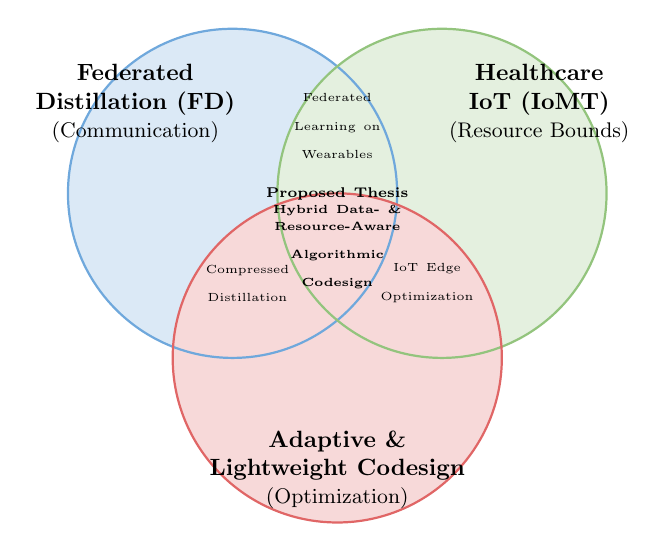
\begin{tikzpicture}[scale=0.95, every node/.style={scale=0.85}, line join=round, line cap=round]
    % Define custom harmonious pastel colors
    \definecolor{colorfd}{RGB}{111,168,220}   % Soft blue
    \definecolor{coloriot}{RGB}{147,196,125}  % Soft green
    \definecolor{colorcodesign}{RGB}{224,102,102} % Soft red/rose

    % Fills with high transparency for neat overlap mixing
    \fill[colorfd!25] (0,0) circle (2.2cm);
    \fill[coloriot!25] (2.8,0) circle (2.2cm);
    \fill[colorcodesign!25] (1.4,-2.2) circle (2.2cm);

    % Draw thin professional borders
    \draw[colorfd, thick] (0,0) circle (2.2cm);
    \draw[coloriot, thick] (2.8,0) circle (2.2cm);
    \draw[colorcodesign, thick] (1.4,-2.2) circle (2.2cm);

    % Circle Labels
    \node at (-1.3, 1.2) [align=center] {\textbf{Federated}\\\textbf{Distillation (FD)}\\\small(Communication)};
    \node at (4.1, 1.2) [align=center] {\textbf{Healthcare}\\\textbf{IoT (IoMT)}\\\small(Resource Bounds)};
    \node at (1.4, -3.7) [align=center] {\textbf{Adaptive \&}\\\textbf{Lightweight Codesign}\\\small(Optimization)};

    % Double Intersections (Peripheral domains in literature)
    \node at (1.4, 0.9) [align=center, text width=2cm] {\tiny Federated Learning on Wearables};
    \node at (0.2, -1.2) [align=center, text width=1.5cm] {\tiny Compressed Distillation};
    \node at (2.6, -1.2) [align=center, text width=1.5cm] {\tiny IoT Edge Optimization};

    % Core Triple Intersection (Your Research Question sits here!)
    \node at (1.4, -0.6) [align=center, text width=2.4cm] {
        \fontsize{6.5pt}{8pt}\selectfont
        \keyterm{Proposed Thesis}\\
        \fontsize{5.5pt}{7pt}\selectfont
        \textbf{Hybrid Data- \&}\\
        \textbf{Resource-Aware}\\
        \textbf{Algorithmic Codesign}
    };
\end{tikzpicture}

    \end{columns}
\end{frame}

% Slide 3: Literature Survey & Mind Map
\begin{frame}{Literature Landscape \& High-Level Mind Map}
    \begin{columns}[T]
        \column{0.5\textwidth}
        \textbf{Literature Survey Key Findings}
        \begin{itemize}
            \item Audited 27 papers spanning edge optimization, model compression, and clinical healthcare systems.
            \item Identified the \keyterm{Compression-Utility Trade-off} as a significant gap: static baseline algorithms destroy fine-grained activity recognition features.
            \item Created a detailed hierarchical taxonomy of literature gaps and hardware limits.
        \end{itemize}

        \column{0.5\textwidth}
        \centering
        \textbf{Taxonomy Mind Map Preview}
        \vspace{0.2cm}

        \begin{block}{Interactive Mind Map Access}
            The full interactive mind map is hosted on your research space. Access full links or local documentation in the workspace.
        \end{block}

        \vspace{0.2cm}
        % User Placeholder for Mind Map Screenshot
        \begin{center}
            \setlength{\fboxrule}{0.5pt}
            \fbox{
                \begin{minipage}{0.8\textwidth}
                    \centering
                    \vspace{0.4cm}
                    \fontsize{7pt}{9pt}\selectfont
                    \texttt{[Placeholder: Replace with mind map graphic]} \\
                    \vspace{0.1cm}
                    \texttt{https://github.com/your-org/mindmap}
                    \vspace{0.4cm}
                \end{minipage}
            }
        \end{center}
    \end{columns}
\end{frame}

% Slide 4: Systems & Cloud Infrastructure
\begin{frame}{Systems \& Infrastructure Milestones}
    \begin{block}{AWS Certified Solutions Architect - Associate}
        Successfully achieved the AWS Solutions Architect certification. Validates core competencies in scalable compute clusters, secure multi-tenant network designs, and low-latency storage architectures.
    \end{block}

    \vspace{0.3cm}
    \textbf{Research Workspace Infrastructures}
    \begin{itemize}
        \item Created a dedicated research GitHub organization to host all simulation repositories and ensure complete reproducibility.
        \item Mapped global server aggregation mechanisms to AWS EC2 instance scaling to ensure our edge simulation matches real-world cloud architectures.
    \end{itemize}
\end{frame}

% Slide 5: FL Simulation & Baseline Replication
\begin{frame}[fragile]{FL Framework Decision \& Baseline Replication}
    \begin{columns}[T]
        \column{0.5\textwidth}
        \textbf{Flower Simulation Framework}
        \begin{itemize}
            \item Formally selected \keyterm{Flower} as our FL simulation engine.
            \item Chosen for its modular client-side orchestrations and native support for heterogeneous IoT nodes.
        \end{itemize}

        \vspace{0.2cm}
        \textbf{Baseline Algorithmic Replications}
        \begin{itemize}
            \item Successfully replicated classic Federated Averaging (\texttt{FedAvg}) and Federated Proximal (\texttt{FedProx}) on local hardware.
        \end{itemize}

        \column{0.5\textwidth}
        \centering
        \begin{table}
            \centering
            \caption{Local Baseline Replication Setup}
            \begin{tabular}{lcc}
                \toprule
                \textbf{Parameter} & \textbf{FedAvg} & \textbf{FedProx} \\
                \midrule
                Local Epochs & $5$ & $5$ \\
                Optimizer & SGD & SGD \\
                Proximal Penalty ($\mu$) & -- & $0.01$ \\
                Status & Replicated & Replicated \\
                \bottomrule
            \end{tabular}
        \end{table}
    \end{columns}
\end{frame}

% Slide 6: Next Steps & Challenges
\begin{frame}{Next Steps \& Expected Challenges}
    \textbf{Immediate Objectives (Week 2)}
    \begin{itemize}
        \item Formulate the exact mathematical metrics for client-side data complexity (such as class-based Shannon entropy or Earth Mover's Distance).
        \item Define the data-aware decision tree logic within the adaptive controller.
    \end{itemize}

    \vspace{0.3cm}
    \textbf{Key Expected Challenges}
    \begin{itemize}
        \item Preserving critical activity recognition features under highly skewed patient datasets (statistical non-IID conditions) without violating privacy boundaries.
    \end{itemize}
\end{frame}

% Slide 7: Q&A / Standout Frame
\begin{frame}[standout]
    Thank You!
    \vspace{0.5cm}

    \begin{center}
        \large Questions \& Answers
    \end{center}
\end{frame}

\end{document}
